
In cheminformatics (esp. drug design literature) fingerprints are binary vectors used to determine molecular similarity. For example, FP2 fingerprint is a  1024 bit fingerprint:
\begin{center}
\only<2>{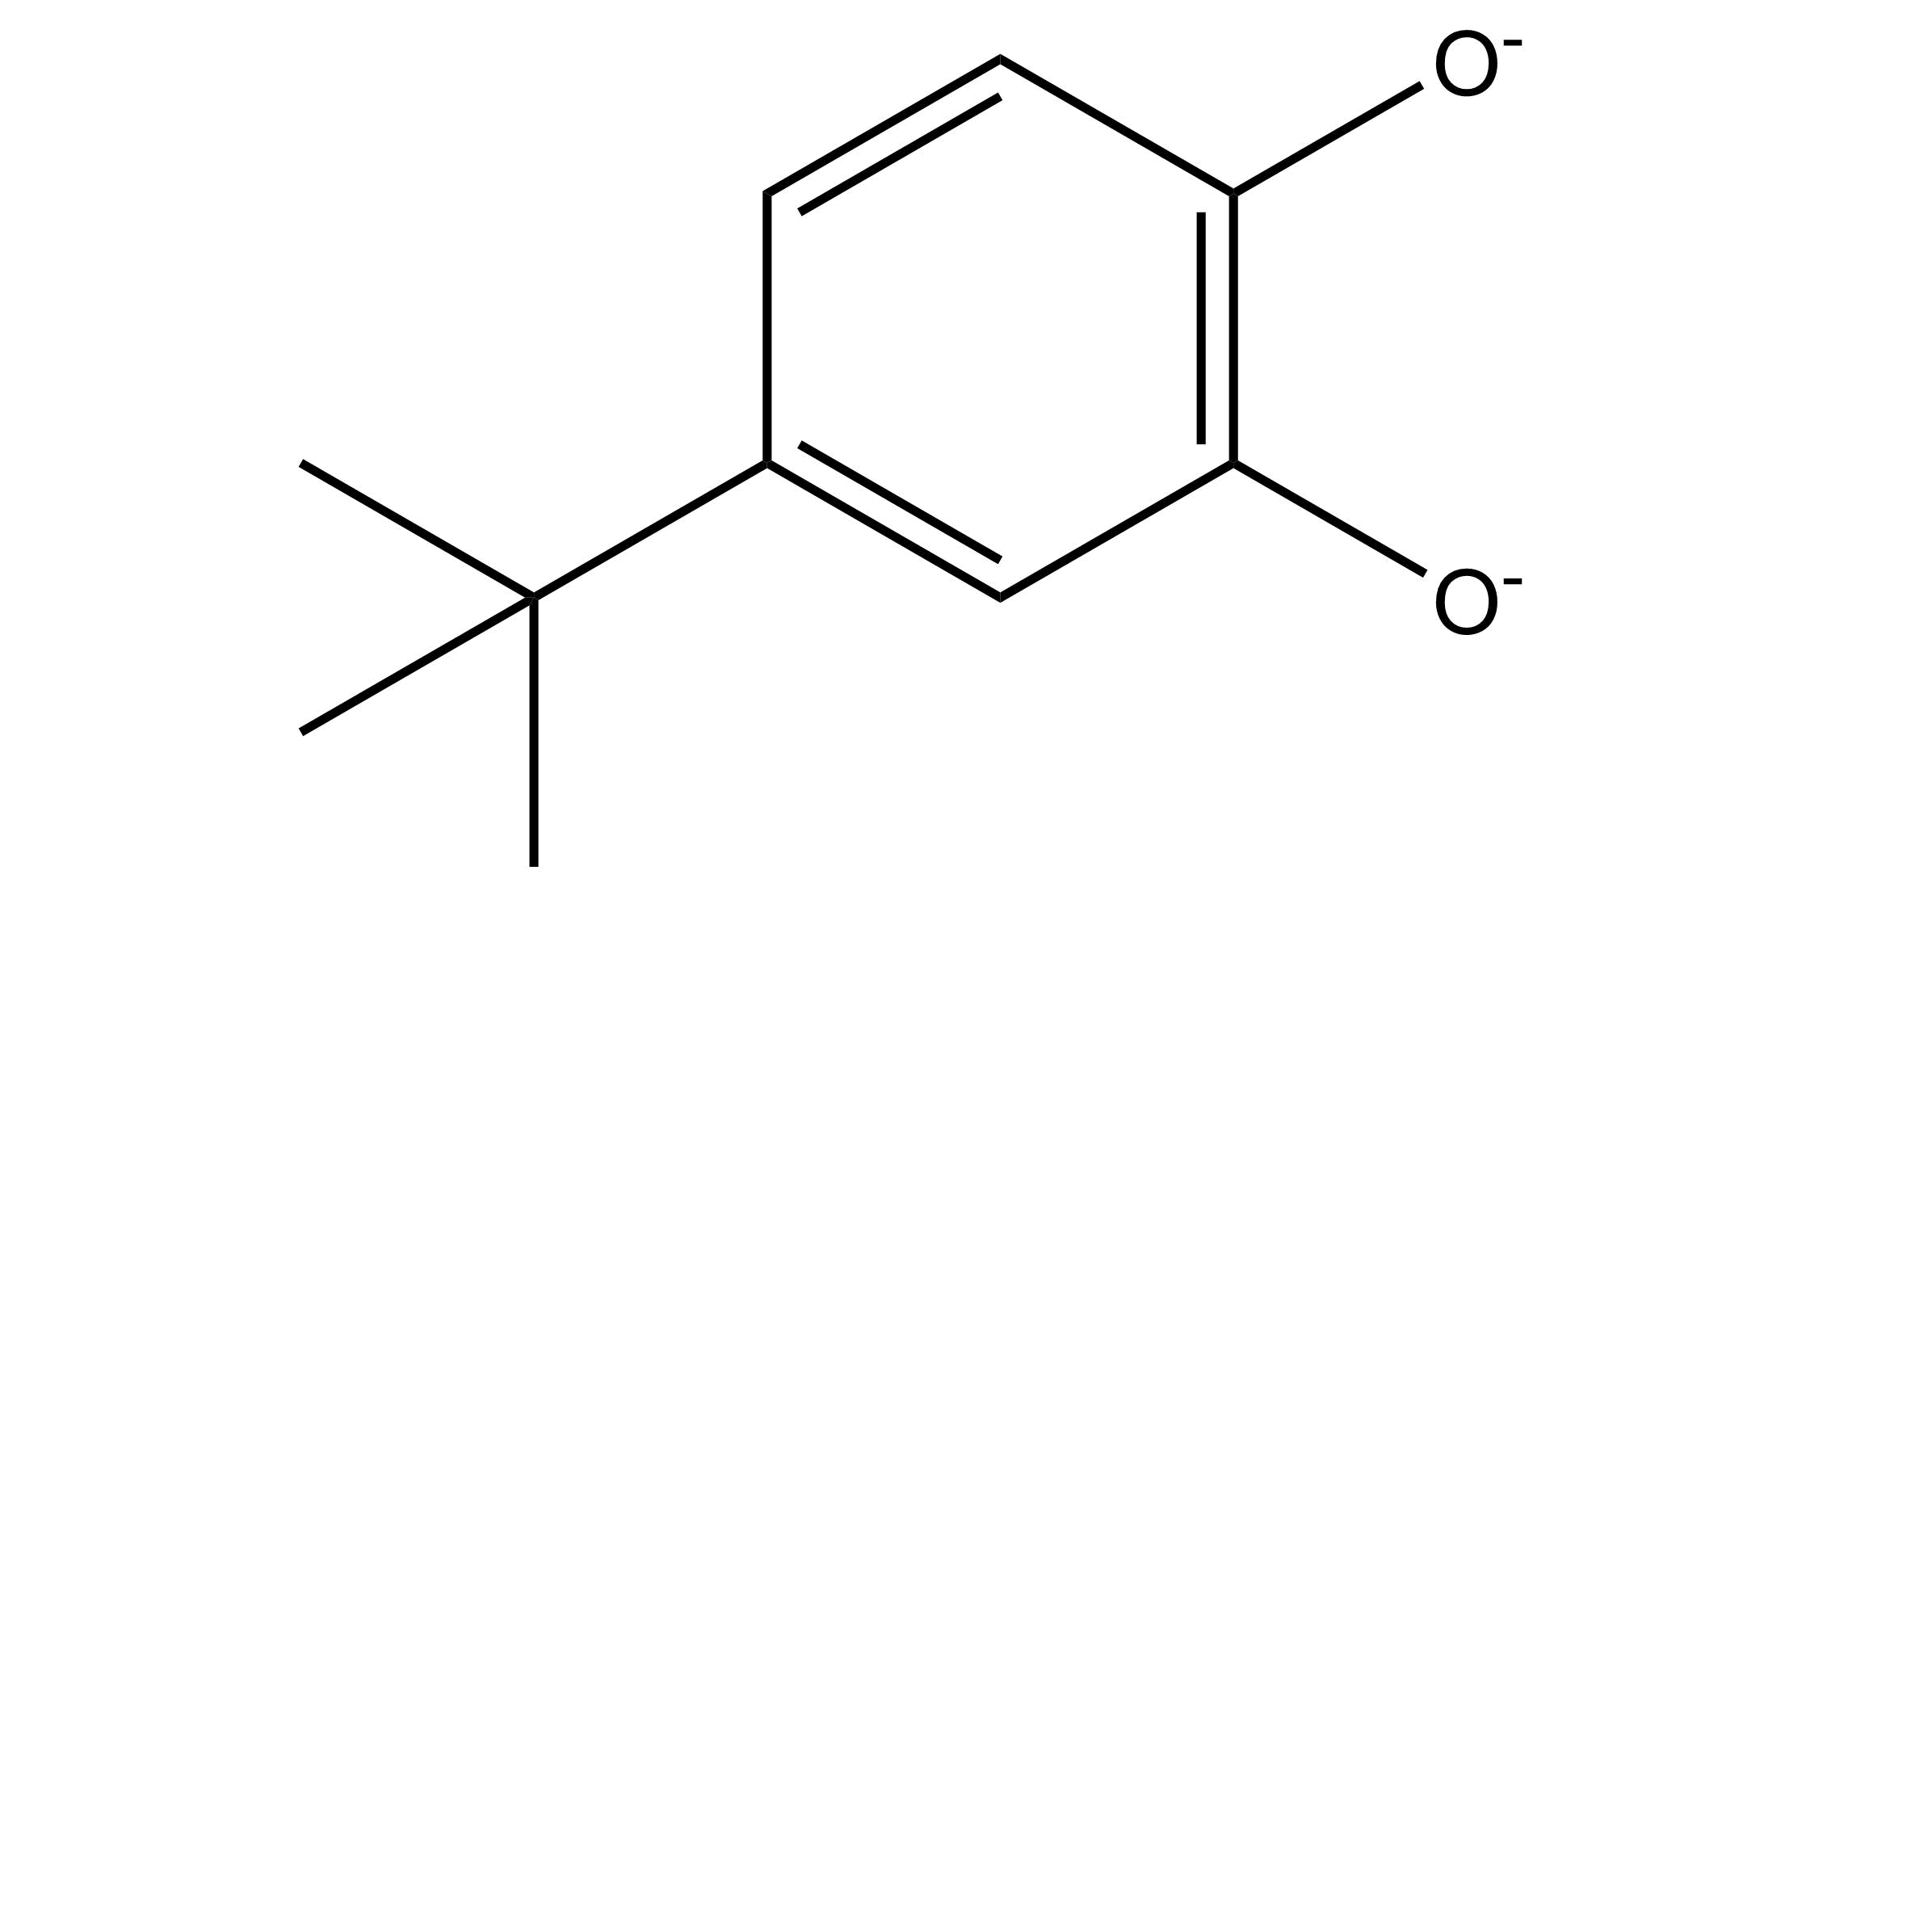
\includegraphics[width=5cm]{representations/images/tbb.png}}
\only<3>{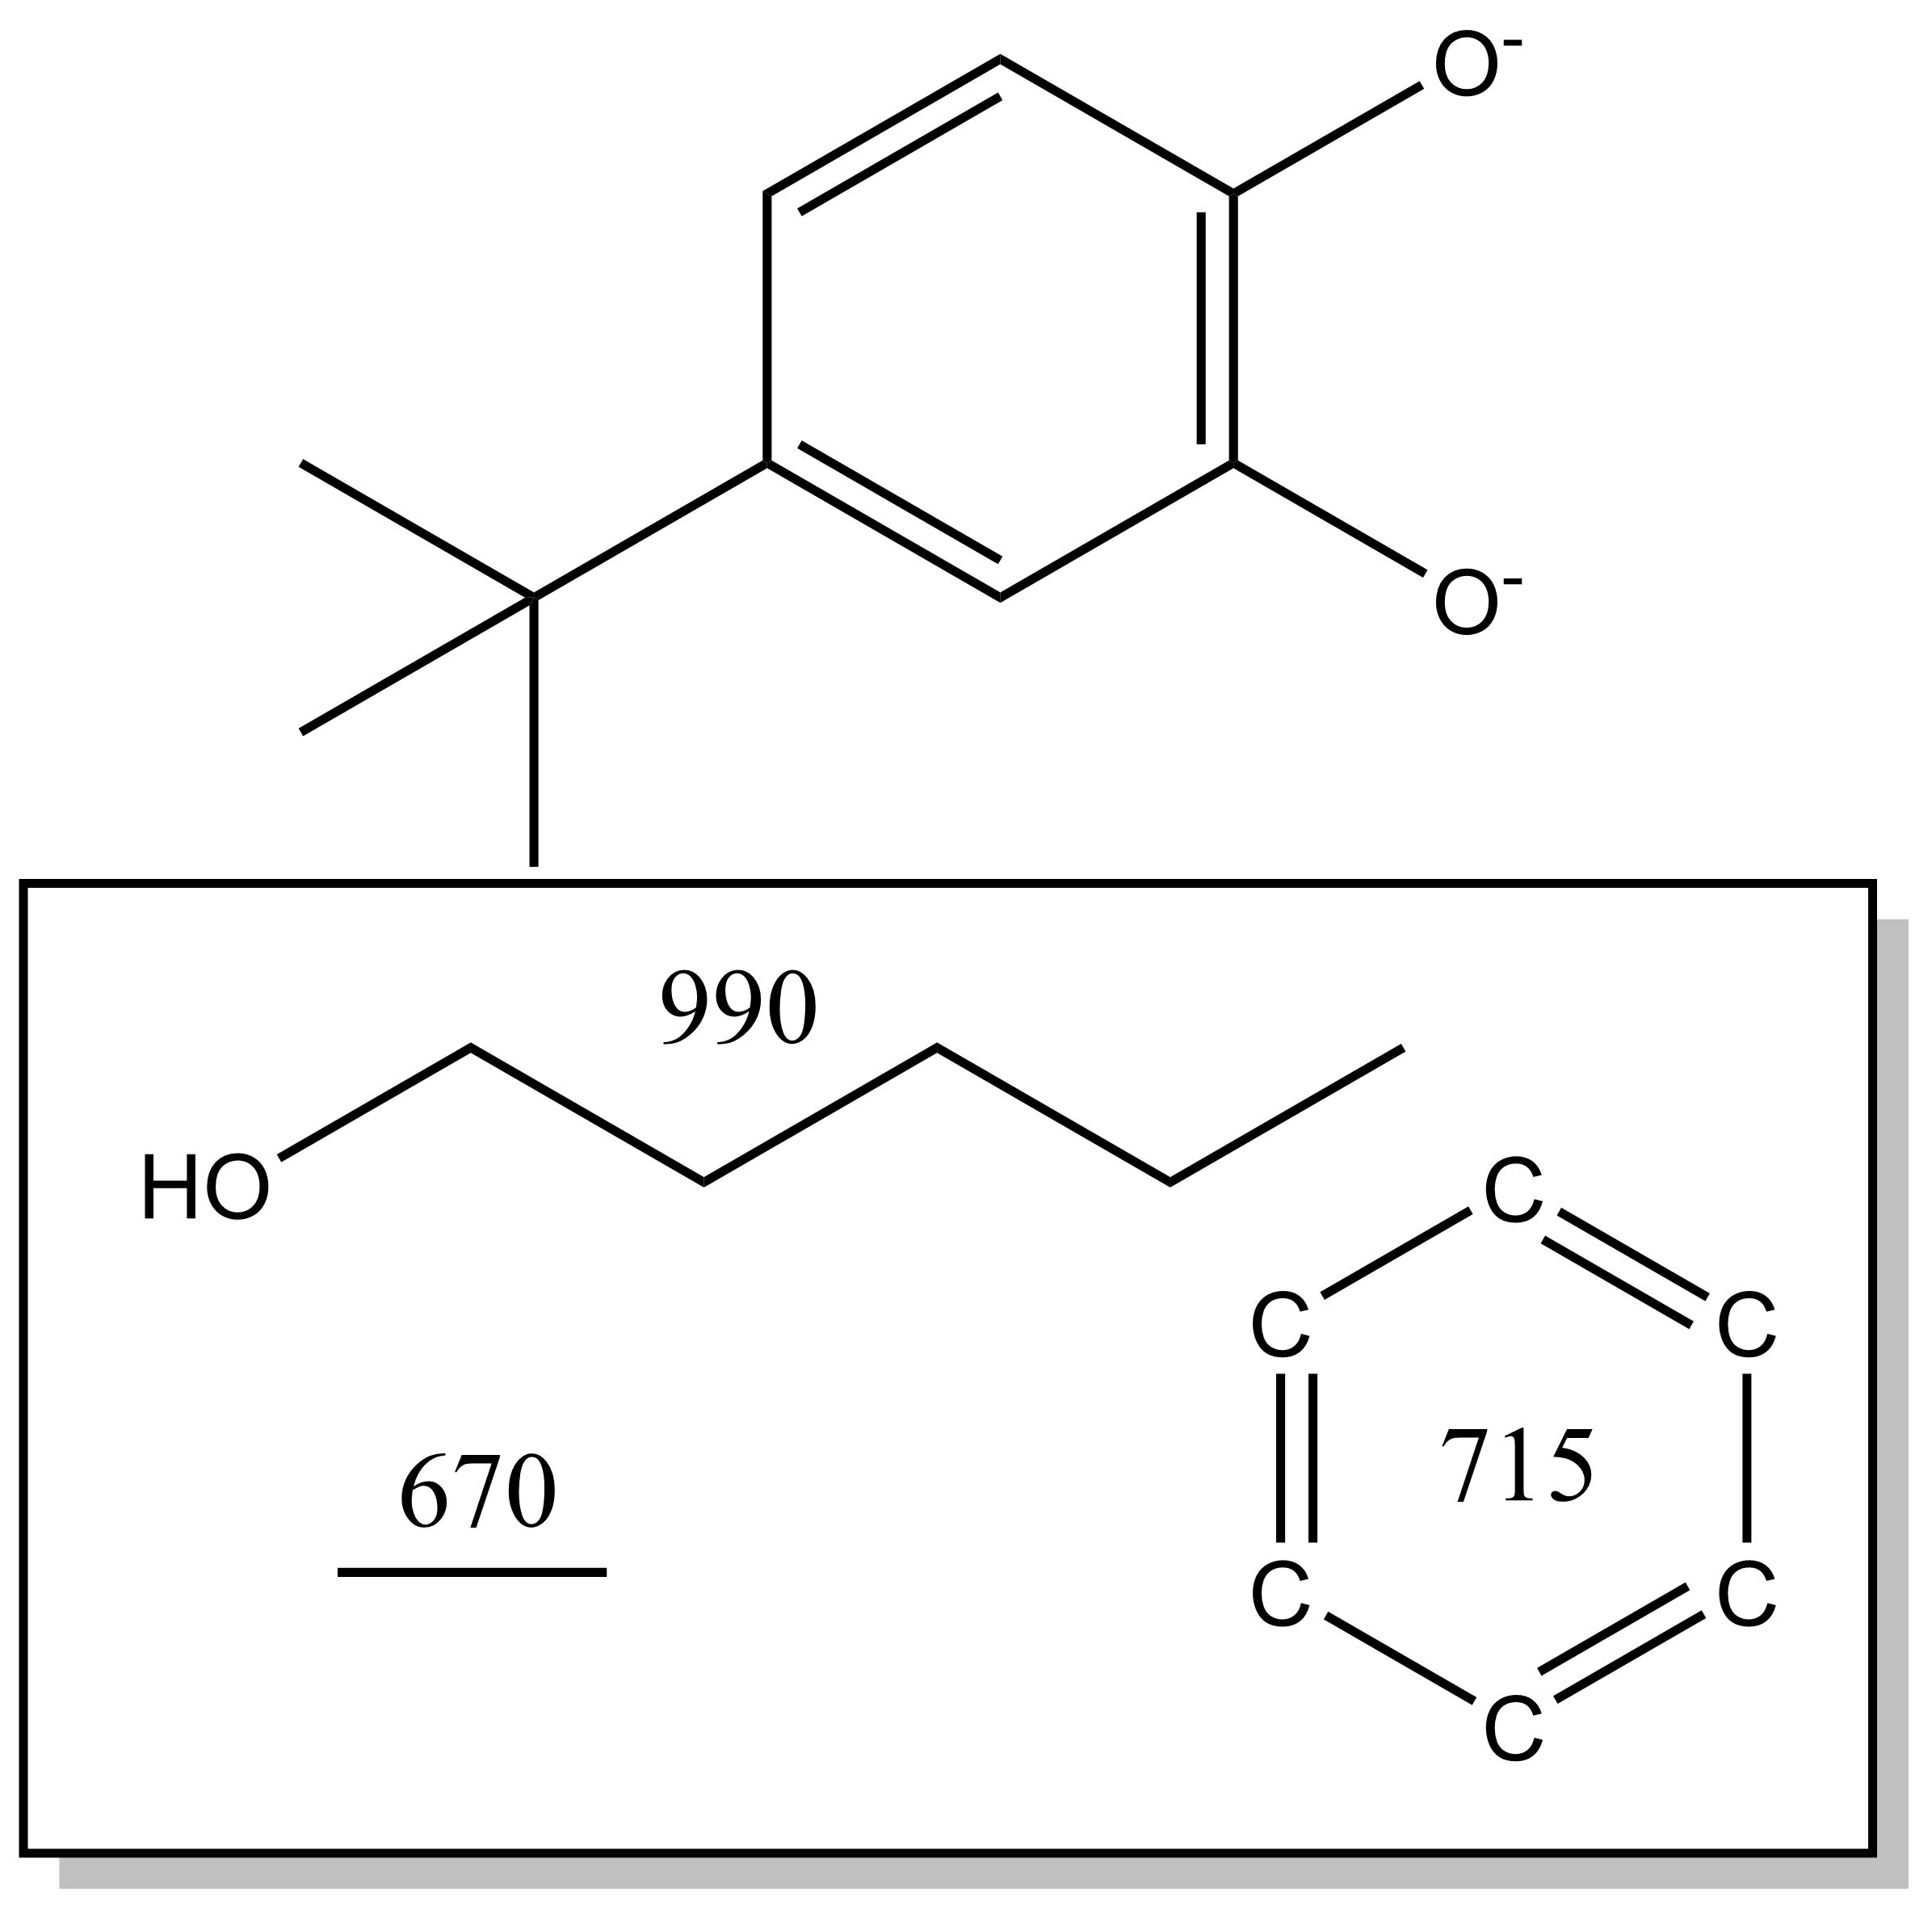
\includegraphics[width=5cm]{representations/images/tb.png}}
\only<4>{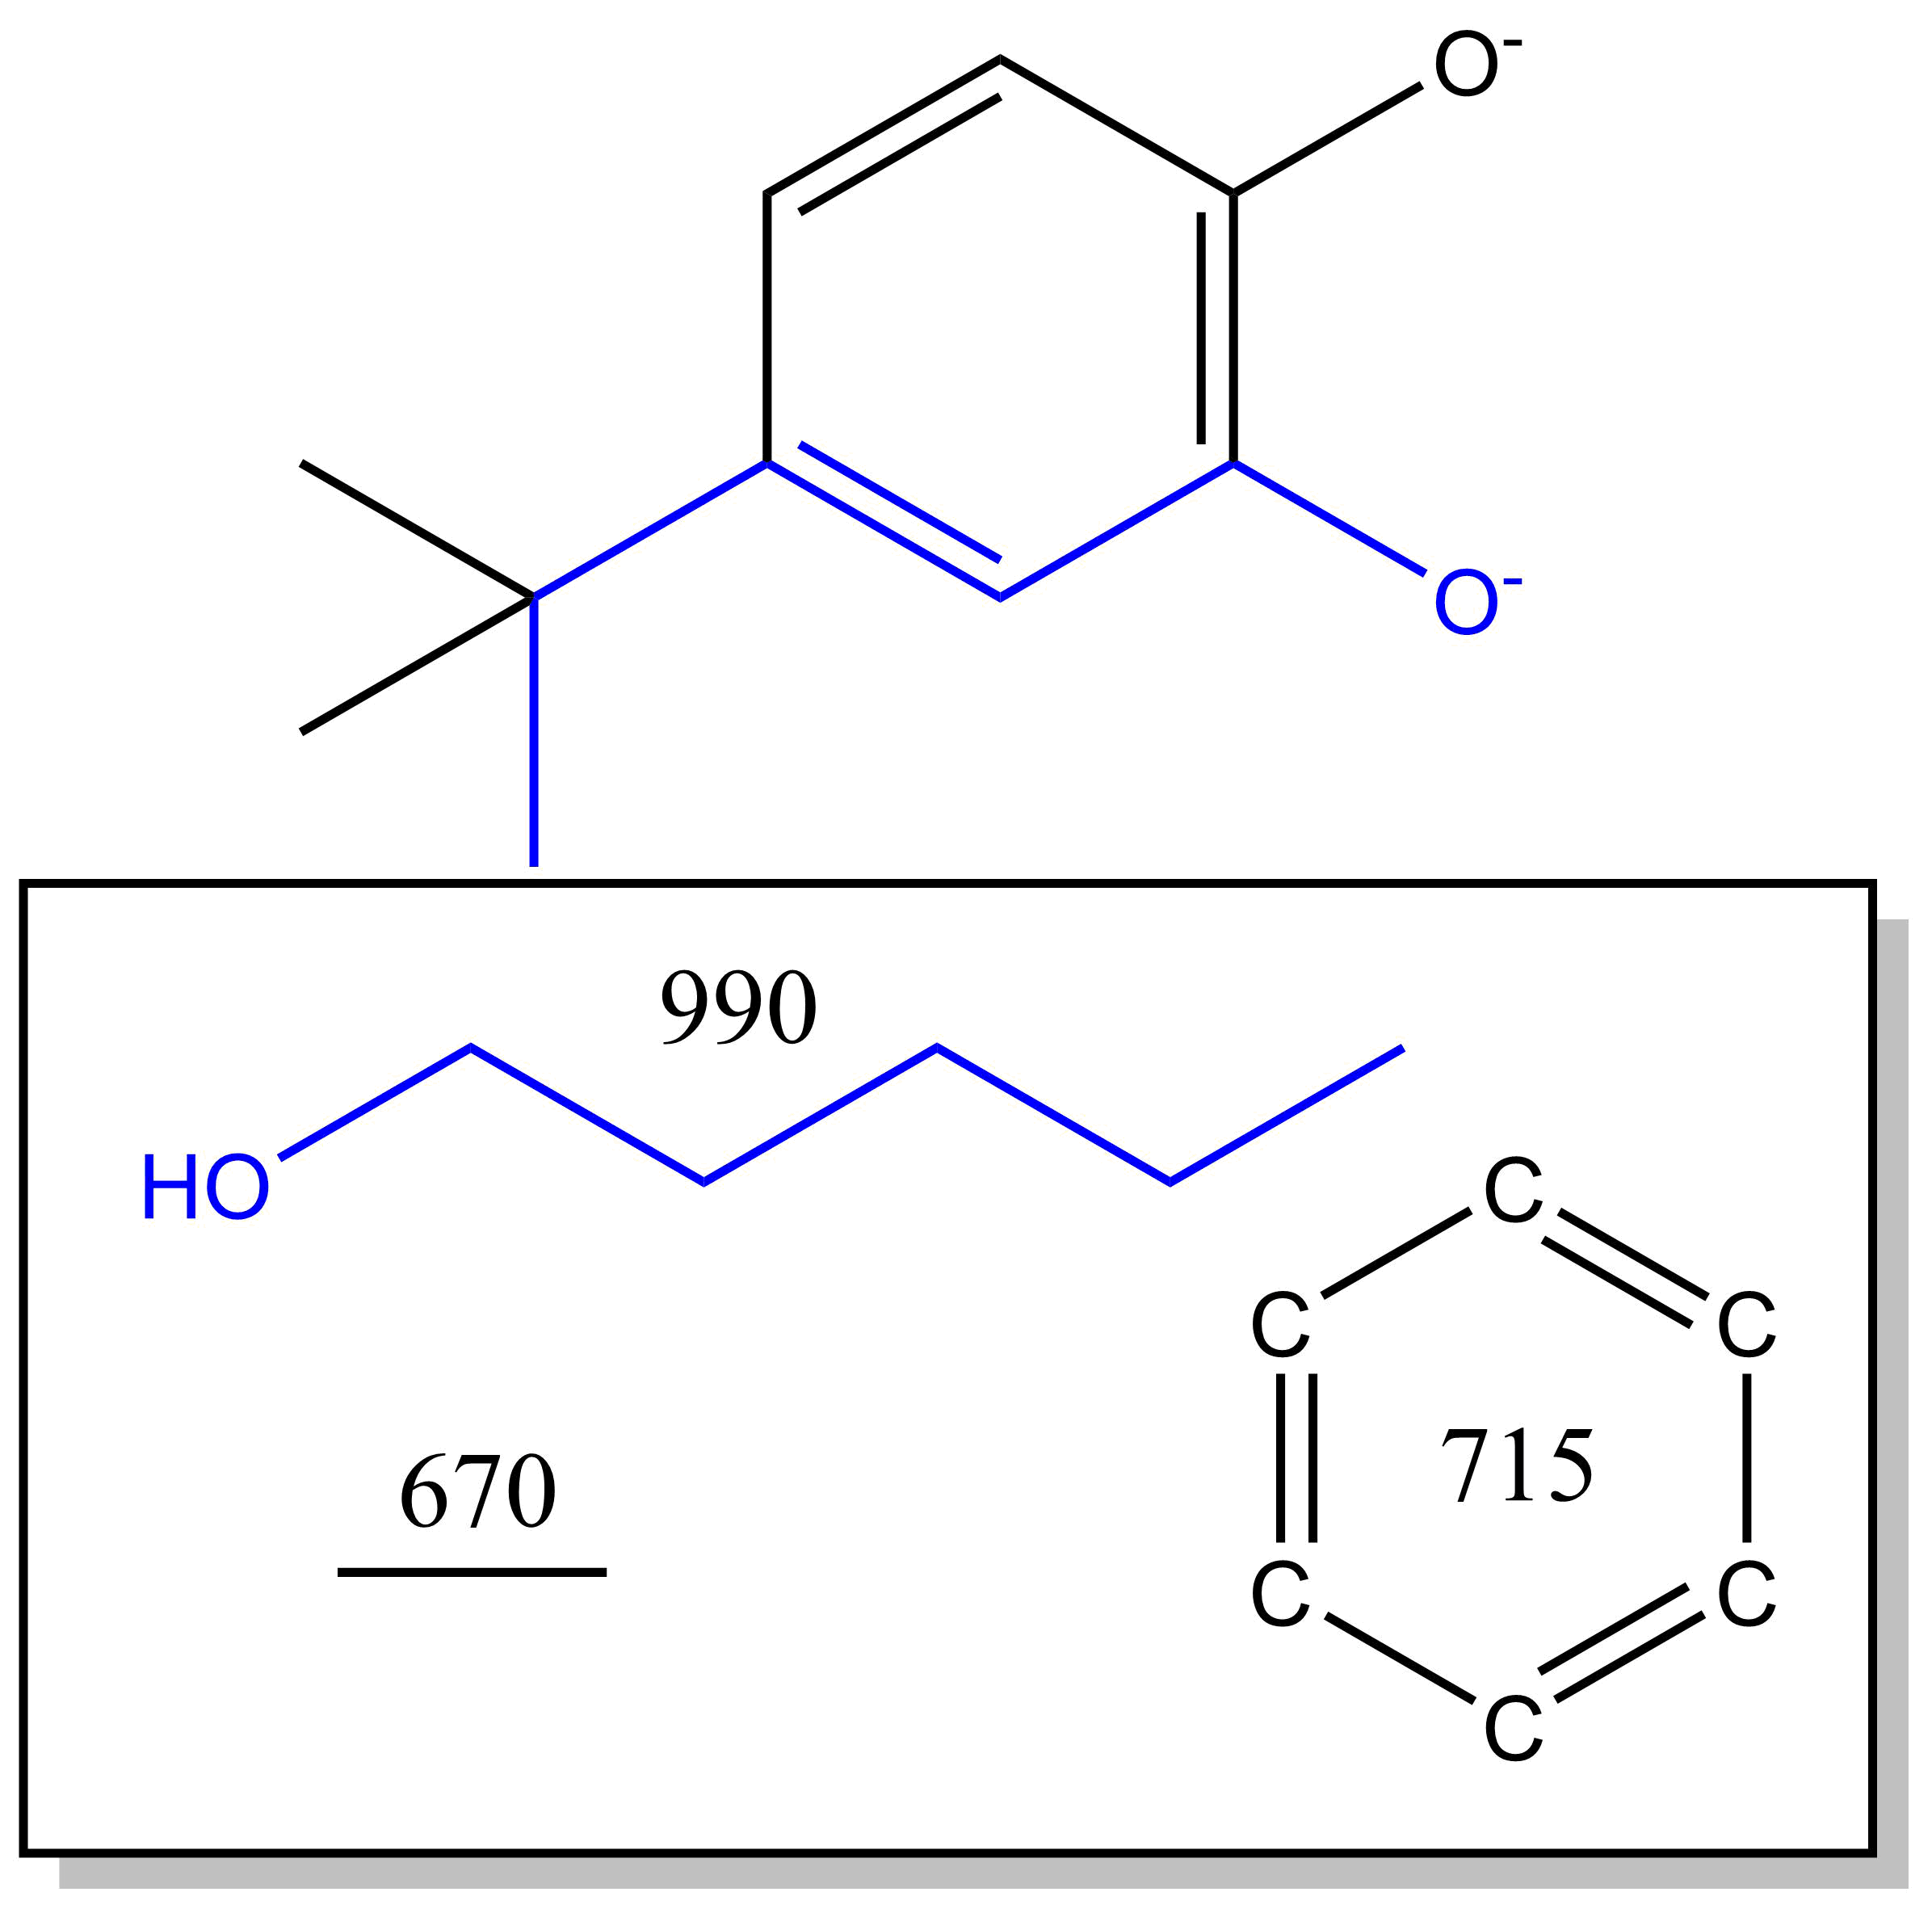
\includegraphics[width=5cm]{representations/images/tbc.png}}
\end{center}



